\documentclass[12pt,letter]{article}
\usepackage[moduleName={Infinite Stairs}]{KautenjaDSP}
\begin{document}
\titlePage{img/Logo}{img/Module}{img/KautenjaDSP}

% -------------------
% MARK: Overview
% -------------------

\section{Overview}

Infinite Stairs is an emulation of the Ricoh 2A03 sound chip from the Nintendo Entertainment System (NES). The 2A03 chip contains two pulse wave generators, a quantized triangle wave generator, and a noise generator. The original chip featured a DMC loader for playing samples that has been omitted in this emulation. Infinite Stairs provides the key features of the 2A03 chip, namely,
\begin{itemize}
  \item \textbf{Dual pulse wave generator:} Dual pulse waveform generator with duty cycles of $12.5\%$, $25\%$, $50\%$, and $75\%$; and 10-bit frequency value
  \item \textbf{Quantized triangle wave generator:} triangle waveform generator with 11-bit frequency value and 16 steps of quantization
  \item \textbf{Noise generator:} generate pseudo-random numbers at 16 different frequencies
  \item \textbf{4-bit Amplifier:} A 4-bit amplifier controls the output level of each oscillator with base/attenuator knobs and CV inputs (with exception of the triangle waveform, which always emits at max volume)
  \item \textbf{Channel Mixer:} Mix the voices together internally with hard clipping and intentional aliasing
\end{itemize}

% -------------------
% MARK: Panel Layout
% -------------------

\clearpage
\section{Panel Layout}

\begin{figure}[!htp]
\centering
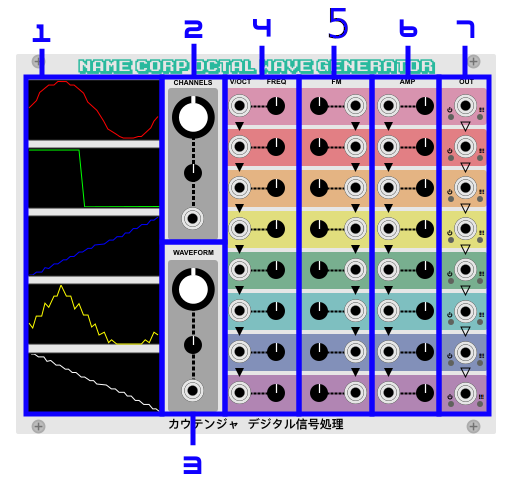
\includegraphics{img/Interface}
\end{figure}

\subsection{Frequency}

The trimpot controls the coarse frequency of the three waveform generators. Frequency is quantized to a 10-bit value for the pulse waveform generators and an 11-bit value for the triangle waveform generator, which is particularly noticeable in the very low / high registers. The ports provide an exponential $V$/Octave input for controlling the pitch of the waveform generators. Inputs are normalled forward from Tone 1, to Tone 2, to Triangle.

\subsection{Frequency Modulation}

When nothing is patched to the frequency modulation port, the trimpot can be used to fine tune the frequency of the given waveform generator. When a signal is patched, the input port provides linear frequency modulation to the corresponding waveform generator and the trimpot can be used as an attenuverter to attenuate / polarize the incoming signal. Inputs are normalled forward from Tone 1, to Tone 2, to Triangle, and support audio rates.

\subsection{Noise}

The trimpot controls the \textbf{period} of the noise generator $\in [0, 15]$. Table~\ref{tab:noise-periods} describes a mapping between the discrete options and fundamental frequencies / MIDI notes. When an input is patched to the port, the CV controls the offset from the trimpot's position. The position of the knob is offset by the CV in increments of $0.5V$. When the \textbf{LFSR} switch is pointing up, the noise generator produces periodic noise. When pointing down, pitched white noise is generated. The input port acts like a gate that goes high at $2V$ and inverts the value of the LFSR switch.

\begin{table}[!htp]
\centering
\caption{A mapping of each noise period to sample rate, fundamental frequency, and MIDI note.}
\label{tab:noise-periods}
\begin{tabular}{|c||r|r|r|}
\hline
 \bfseries Period  & \bfseries Sample Rate ($Hz$) & \bfseries Fundamental ($Hz$)   & \bfseries MIDI note       \\
\hline\hline
 0       & $447443.2$         & $4811.2$             & \texttt{110.41} \\
\hline
 1       & $223721.6$         & $2405.6$             & \texttt{98.41}  \\
\hline
 2       & $111860.8$         & $1202.8$             & \texttt{86.41}  \\
\hline
 3       & $55930.4$          & $601.4$              & \texttt{74.41}  \\
\hline
 4       & $27965.2$          & $300.7$              & \texttt{62.41}  \\
\hline
 5       & $18643.5$          & $200.5$              & \texttt{55.39}  \\
\hline
 6       & $13982.6$          & $150.4$              & \texttt{50.41}  \\
\hline
 7       & $11186.1$          & $120.3$              & \texttt{46.55}  \\
\hline
 8       & $8860.3$           & $95.3$               & \texttt{42.51}  \\
\hline
 9       & $7046.3$           & $75.8$               & \texttt{38.55}  \\
\hline
 10      & $4709.9$           & $50.6$               & \texttt{31.57}  \\
\hline
 11      & $3523.2$           & $37.9$               & \texttt{26.55}  \\
\hline
 12      & $2348.8$           & $25.3$               & \texttt{19.53}  \\
\hline
 13      & $1761.6$           & $18.9$               & \texttt{14.55}  \\
\hline
 14      & $879.9$            & $9.5$                & \texttt{2.53}   \\
\hline
 15      & $440.0$            & $4.7$                & \texttt{-9.47}  \\
\hline
\end{tabular}
\end{table}

\subsection{Amplifier}

When no input is connected, the trimpot controls the given waveform generator volume level with 4-bit resolution (i.e., $\in [0, 15]$). When an input is patched to the port, the trimpot acts like an attenuator that scales the CV control over the volume level. Because the amplifier has 4-bit control, the envelope of the voice will sound quantized when used with an external envelope generator. Inputs are normalled forward from Tone 1, to Tone 2, to Noise.

\subsection{Pulse Width}

The trimpot chooses between four duty cycles: $12.5\%$, $25\%$, $50\%$, and $75\%$. When an input is patched to the port, the CV controls the offset from the trimpot's position. The position of the knob is offset by the CV in increments of $2V$.

\subsection{Sync}

The sync inputs can be used to manually reset either the triangle waveform or noise generators to synchronize with another oscillator. These ports support audio rate modulation.

\subsection{Outputs}

Each voice produces an output signal of at most $10V_{pp}$ when the amplifier is maxed out. The individual oscillators cannot be overdriven to produce clipping, distortion, or aliasing. However, outputs are normalled forward into a sum mix where hard clipping \textit{can} occur. Excess clipping will introduce an aliasing effect to the mix. Outputs in the mix are clipped \textit{before} being normalled to the next output. VU meter lights measure the output of individual channels going from off ($-\infty dB$ to $-12dB$), to green ($-12dB$ to $0dB$), and lastly to red ($0dB$ to $3dB$) when clipping begins to occur.

% -------------------
% MARK: Data Sheet
% -------------------

\clearpage
\section{Data Sheet}

\begin{table}[!htp]
\begin{tabular}{|l|l|}
\hline
Type             & Oscillator               \\
\hline
Size             & 10 HP Eurorack           \\
\hline
Depth            & NA                       \\
\hline
Power            & NA                       \\ % 2 x 5 Eurorack
\hline
$+12V$ draw (mA) & 0 mA                     \\
\hline
$-12V$ draw (mA) & 0 mA                     \\
\hline
$+5V$ draw (mA)  & 0 mA                     \\
\hline
Sample Rate      & Programmable             \\
\hline
Bit Depth        & 16-bit                   \\
\hline
\end{tabular}
\end{table}

% -------------------
% MARK: References
% -------------------

\clearpage
\renewcommand\refname{References}
\nocite{*}
\bibliographystyle{apalike}
\bibliography{references}

\end{document}
